\documentclass{article}
\usepackage[utf8]{inputenc}
\usepackage{graphicx}
\usepackage{subcaption}
\usepackage[export]{adjustbox}
\usepackage{wrapfig}
\title{Extrapolating NBA Career Trajectories From Rookie Year Stats}
\author{Akash Kumar(ajk279) and Pranav Darbha(pd353)}
\date{\vspace{-5ex}}
\begin{document}

\maketitle

\section{Introduction}
In the annual NBA Draft, 60 players from American universities and other leagues around the world are chosen in the hope that they can be strong players in the world's most competitive basketball league. The volatility of the rookie season can make it difficult to predict how a player will perform further into their NBA career. There are those who succeeded in their first taste of the NBA and never looked back and there are those who have continually regressed since that first year.

With the plethora of NBA data available for draft classes throughout the years, we hope to be able to predict the performance of 2016-17 Rookies in the upcoming season. We plan on using datasets from www.basketball-reference.com containing player statistics from 2010 onwards as well as NBA 2K ratings to measure the overall capability of a player. From basketball-reference, we plan on using both traditional metrics like points, rebounds and assists as well as advanced statistics like Player Efficiency Ratings and Value Over Replacement Player. We will collect this data from the players' rookie years and try to use it to predict their NBA 2K ratings 3 years down the line. We believe 2K ratings are accurate indicators of overall skill because they are meticulously developed to take into account all aspects of a player's game. They are also widely accepted as the video game franchise routinely sells over 10 million copies each year. We decided to use this rating from a model design perspective because we wanted a quantitative way to predict a player's overall future potential rather than classifying them into tiers based on awards or simply predicting specific statistics. Once we have built our predictive model, we can evaluate its performance by looking at the stats of the 2016-17 Rookies in their fourth NBA season, which began recently.
\section{Data and Preprocessing}
As was previously mentioned, we collected a mix of advanced and traditional statistics for each player's rookie and fourth year seasons from basketball-reference.com. Our models are only trained on the players' rookie year statistics to predict the 2k rating, but we collected the statistics for the fourth year as well for us to reference. Figure 1 shows the features that were used and the correlation between them. 
\begin{figure}[htp]
    \centering
    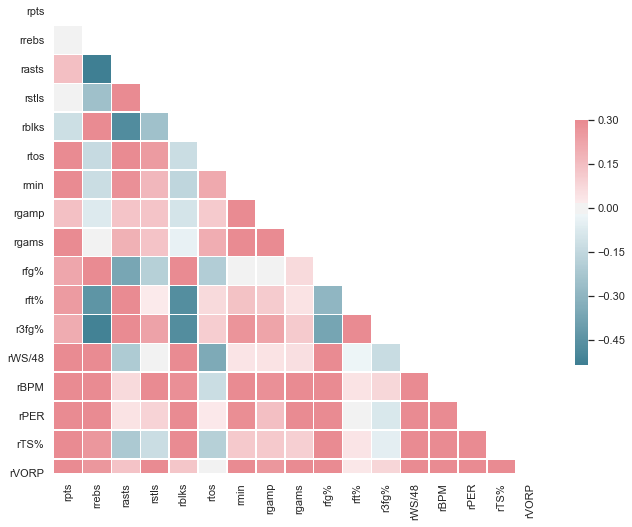
\includegraphics[width=5cm]{feature_heatmap.png}
    \caption{Heatmap showing our features and the correlations to the other features}
\end{figure} 

Our first intuition was to manually label each player by classifying them into 5 tiers. These tiers loosely corresponded to "Bench player", "Rotation player", "Starter", "All-Star caliber", and "All-NBA caliber". We manually labelled them by looking at the accolades and stats they had accrued in their first four years. We initially represented these labels with one-hot vectors, but we saw poor performance from the models because the overwhelmingly high number of Tier 1 players gave us high accuracy models that misclassified many players as Tier 1. We then changed our labels using the encoding style normally used for ordinal data that was shown in class. This change in encoding did not make much of a difference, however, which led to us pivoting and using a regression approach with the NBA 2k ratings rather than a multi-class classification. To collect this data we visited a variety of sites that tracked these ratings and added the ratings to the dataset.
\section{Preliminary Models and Results}
The work discussed in this section can be found in the "2krank predictions.ipynb" file in our GitHub repository. Since we are predicting a quantitative output in 2K rating, we decided that regression was a good place to start. We made sure to split up our data randomly into training and test sets with 20 percent of the data in the test set. This provides us with a way to check if our models are accurate and if they are overfitting or underfitting. We made sure to also scale our features in order to make up for the order of magnitude difference between statistics such as points and VORP. The four main models we tried were Linear Regression, Polynomial Regression, Ridge Regression and Lasso Regression. Results for each are shown below. The graphs all show the predicted vs true values on the test set.
\begin{figure}[h]
\begin{subfigure}{0.5\textwidth}
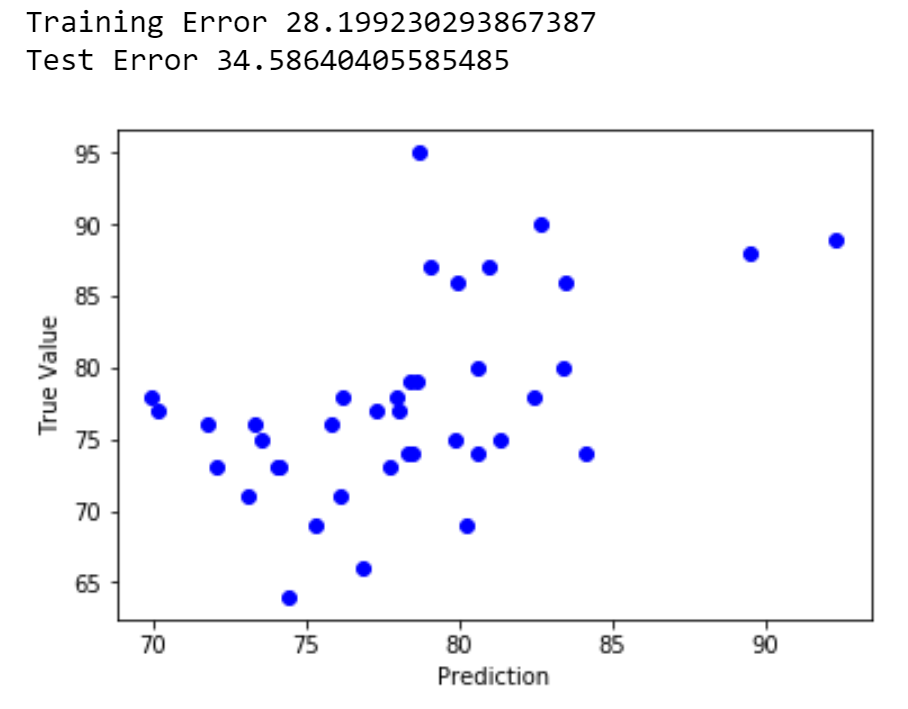
\includegraphics[width=0.9\linewidth]{nbalinreg.png} 
\caption{Linear Regression}
\end{subfigure}
\begin{subfigure}{0.5\textwidth}
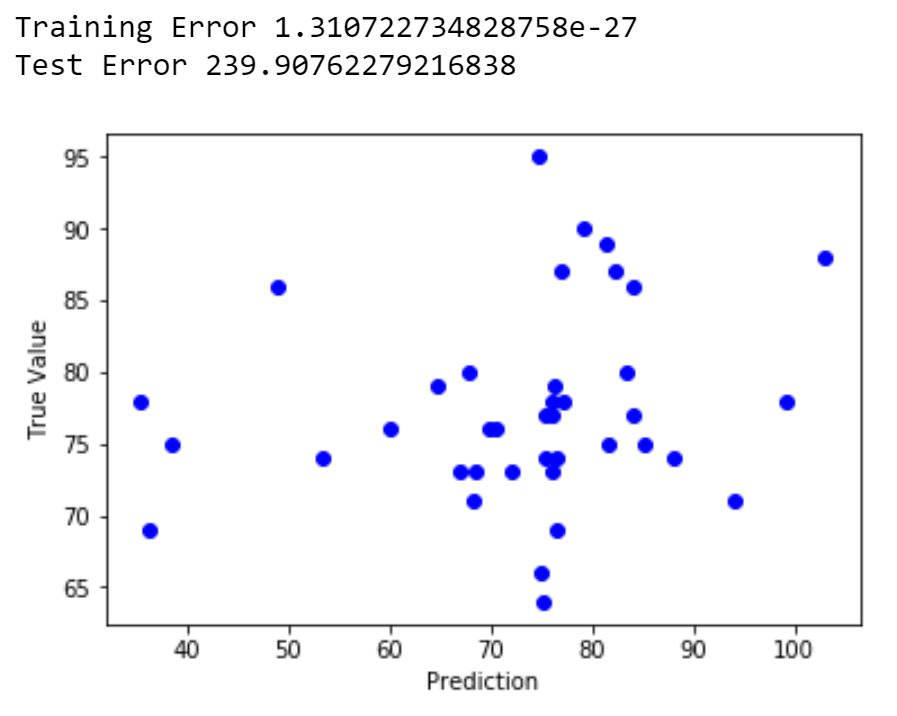
\includegraphics[width=0.9\linewidth]{nbapolyreg.png}
\caption{Polynomial Regression}
\end{subfigure}
\end{figure}
\begin{figure}[h]
\begin{subfigure}{0.5\textwidth}
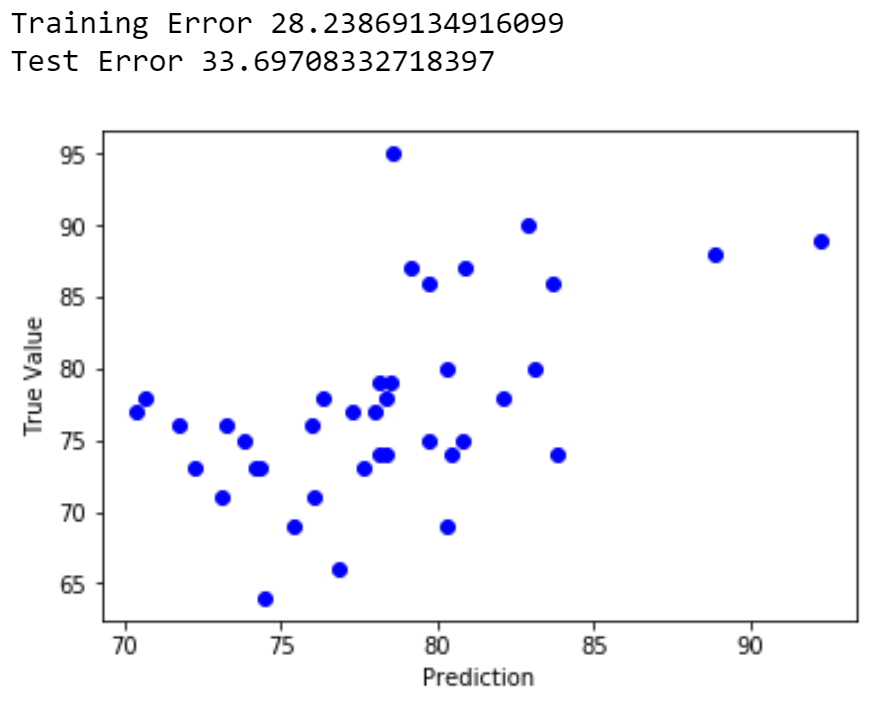
\includegraphics[width=0.9\linewidth]{nbaridgereg.png} 
\caption{Ridge Regression}
\end{subfigure}
\begin{subfigure}{0.5\textwidth}
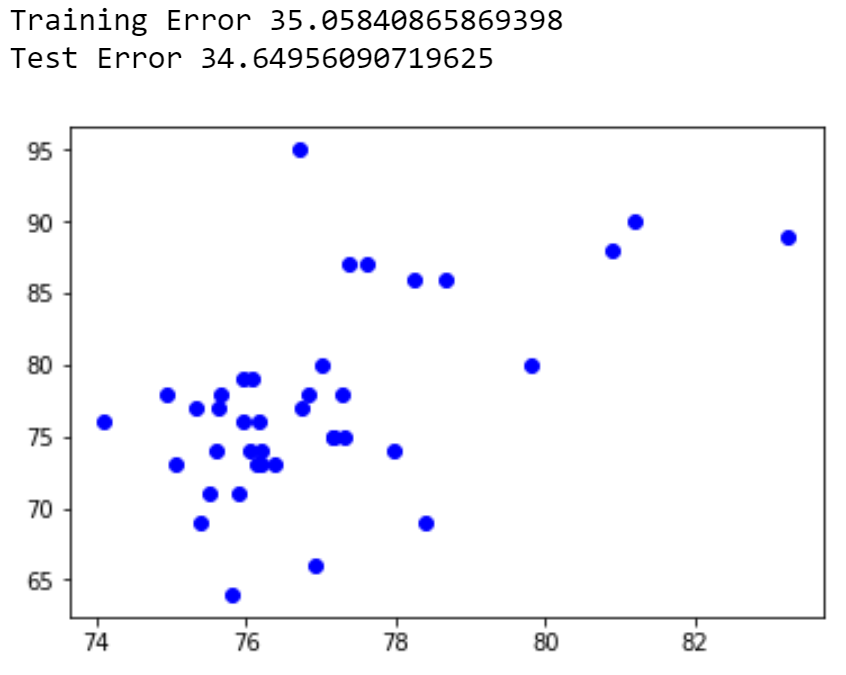
\includegraphics[width=0.9\linewidth]{nbalassoreg.png}
\caption{Lasso Regression}
\end{subfigure}
\end{figure}
From these results, we can notice a few things. First of all, polynomial regression severely overfits our model. The shown graph is with degree 3, but the same result appeared for other degrees. The training error is extremely low while the test error is high. Linear Regression and Ridge Regression appear to be our two best models. Both have mean squared training error around 28 and mean squared test error around 34. Ridge improves slightly on the test error at the expense of some training error and Lasso does worse on both fronts. In the context of our model, this error means that our predictions are, on average, around 5-6 rating points off. This is pretty good for a preliminary analysis, but can definitely be improved upon. 
\section{Takeaways and Ideas for Future}
Based on our results from the tests we ran, it seems that Ridge Regression is the model we will use going forward. In the future, we plan on using cross-validation to tune the hyper-parameters associated with ridge regression (lambda). We may also consider adding more data to potentially correct the overfitting we have seen, but because of the changes in rookie usage over the years as well as the style of basketball in the NBA, old data may not be useful for us.

We may experiment with other models that are not necessarily regression as well. Using neural networks could also help us predict player ratings by generating a 1-dimensional vector. Another way of looking at this problem is by considering it a classification problem where the classes include ratings \textless60, 60-65, 65-70, etc. and trying to use a classification algorithm to predict that.
\end{document}